% Intended LaTeX compiler: pdflatex
\documentclass[10pt,a4paper,UTF8]{article}
\usepackage{zclorg}
\usepackage{tikztheorem}
\author{emacsun}
\date{}
\title{漂亮的Emacs 主题}
\hypersetup{
 pdfauthor={emacsun},
 pdftitle={漂亮的Emacs 主题},
 pdfkeywords={},
 pdfsubject={},
 pdfcreator={Emacs 25.0.50.1 (Org mode 9.1.2)},
 pdflang={English}}
\begin{document}

\maketitle
\tableofcontents
\titlepic{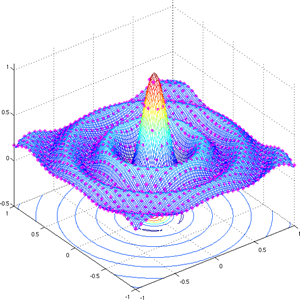
\includegraphics[scale=0.25]{../../img/sinc.PNG}}

\section{Emacs theme gallary}
\label{sec:org4ad18bb}
尽管年老,Emacs也没有停止追求美。众多的Emacs拥趸为Emacs打造不同风格的主题。在 \href{https://emacsthemes.com/index/1.html}{这里} 和 \href{https://pawelbx.github.io/emacs-theme-gallery/}{这里} 保存了一些非常漂亮的Emacs主题。另外, \href{https://draculatheme.com/emacs/}{Dracula} 也是一款比较漂亮的主题。

\section{spacemacs切换主题}
\label{sec:orgb1b5ff2}

我比较喜欢Solarized主题。这个主题有两套一套淡色(solarized-light)的一套深色(solarized-dark)。另外一个比较令我喜欢的是monokai。在spacemacs里可以通过 \texttt{spc T s} 来切换主题。

如果遇到自己比较喜欢的主题可以在 \texttt{init.el} 的 \texttt{dotspacemacs-themes} 变量列表中保存。这样 \texttt{spc T s} 跳出的列表中就会有你喜欢的主题供选择。目前我的列表是:
\begin{verbatim}
dotspacemacs-themes '(
                      monokai
                      solarized-dark
                      monokai
                      spacemacs-dark
                      spacemacs-light
                      solarized-light
                      leuven
                      zenburn)
\end{verbatim}

\section{美化Emacs}
\label{sec:org92a1af2}

\href{http://www.modernemacs.com/}{Modern Emacs} 为Emacs提供了一些列比较系统的美化。包括各种数学符号的显示,Eshell的显示,Magit的显示。看起来非常的赏心悦目。(插播一下,这个博客的主题叫做 \href{https://draculatheme.com/emacs/}{hugo academic} 是我比较喜欢的一款博客主题。)

我个人并不喜欢这些过度的优化,我还是更喜欢最简单直接的文本。萝卜青菜各有所爱,喜欢的朋友可以移步去看看。
\end{document}
